\documentclass[11pt,a4paper]{article}
\usepackage[french]{babel}
\usepackage[T1]{fontenc}
\usepackage{amsmath,amssymb,amsfonts}
\usepackage{geometry}
\geometry{hmargin=2cm,vmargin=2.5cm}
\usepackage{xcolor}
\usepackage{tcolorbox}
\usepackage{graphicx}
\usepackage{booktabs}
\usepackage{hyperref}

% Définition de la charte graphique académique
\definecolor{maincolor}{RGB}{0,51,102}
\definecolor{accentcolor}{RGB}{0,102,153}
\definecolor{boxbg}{RGB}{245,247,250}

\tcbset{
    colback=boxbg,
    colframe=maincolor,
    fonttitle=\bfseries,
    arc=2mm,
    top=3mm,bottom=3mm,left=4mm,right=4mm
}

\hypersetup{
    colorlinks=true,
    linkcolor=maincolor,urlcolor=accentcolor,
    pdftitle={Rapport de Calibration et Estimation de Pose 3D - Fallou DIOUF}
}

\title{
    \vspace{-1cm}
    \textbf{\Large Master Vision et Machine Intelligente (VMI 2026)}\\
    \rule{\linewidth}{1pt}\\[0.3cm]
    \Huge \textbf{Rapport de Calibration d'un Capteur Passif \& Estimation de Pose 3D}\\[0.2cm]
    \large Traitement d'Image et Vision (TICV2026) -- Rendu 1
    \rule{\linewidth}{1pt}
}
\author{\textbf{Fallou DIOUF}}
\date{\today}

\begin{document}

\maketitle

\begin{abstract}
\noindent Ce rapport documente l'étalonnage géométrique (calibration) complet d'un capteur optique passif (caméra de smartphone) ainsi que l'estimation de sa pose tridimensionnelle (PnP). L'expérimentation s'appuie sur la génération et l'affichage d'un motif théorique $7 \times 10$ ($9 \times 6$ coins internes) généré via la plateforme \texttt{calib.io}. Une série de 19 clichés sous des angles et orientations variés a été acquise. La résolution du système par moindres carrés et SVD sous OpenCV a permis d'extraire la matrice intrinsèque $K$, les coefficients de distorsion, l'erreur RMS ($2{,}42\text{ pixels}$) et la longueur focale physique exprimée en mètres ($f = 0{,}004789\text{ m}$) via la fonction \texttt{calibrationMatrixValues()}.
\end{abstract}

\vspace{0.5cm}

\section{Protocole Expérimental \& Génération du Motif}

\subsection{Génération du Motif via \texttt{calib.io}}
Pour garantir une géométrie parfaite du motif sans déformation d'impression papier, le motif de calibration a été généré depuis la plateforme spécialisée \textbf{calib.io} (\textit{Camera Calibration Pattern Generator}). Les paramètres de configuration choisis sont les suivants :
\begin{itemize}
    \item \textbf{Target Type :} \texttt{Checkerboard} (Damier).
    \item \textbf{Dimensions globales :} $200\text{ mm} \times 150\text{ mm}$.
    \item \textbf{Grille (Lignes $\times$ Colonnes) :} $7 \times 10$ carrés, ce qui correspond rigoureusement à $(10-1) \times (7-1) = \mathbf{9 \times 6}$ \textbf{coins internes} (intersections recherchées par l'algorithme).
    \item \textbf{Checker Size (Taille théorique) :} $15\text{ mm}$.
\end{itemize}

\begin{figure}[ht!]
    \centering
    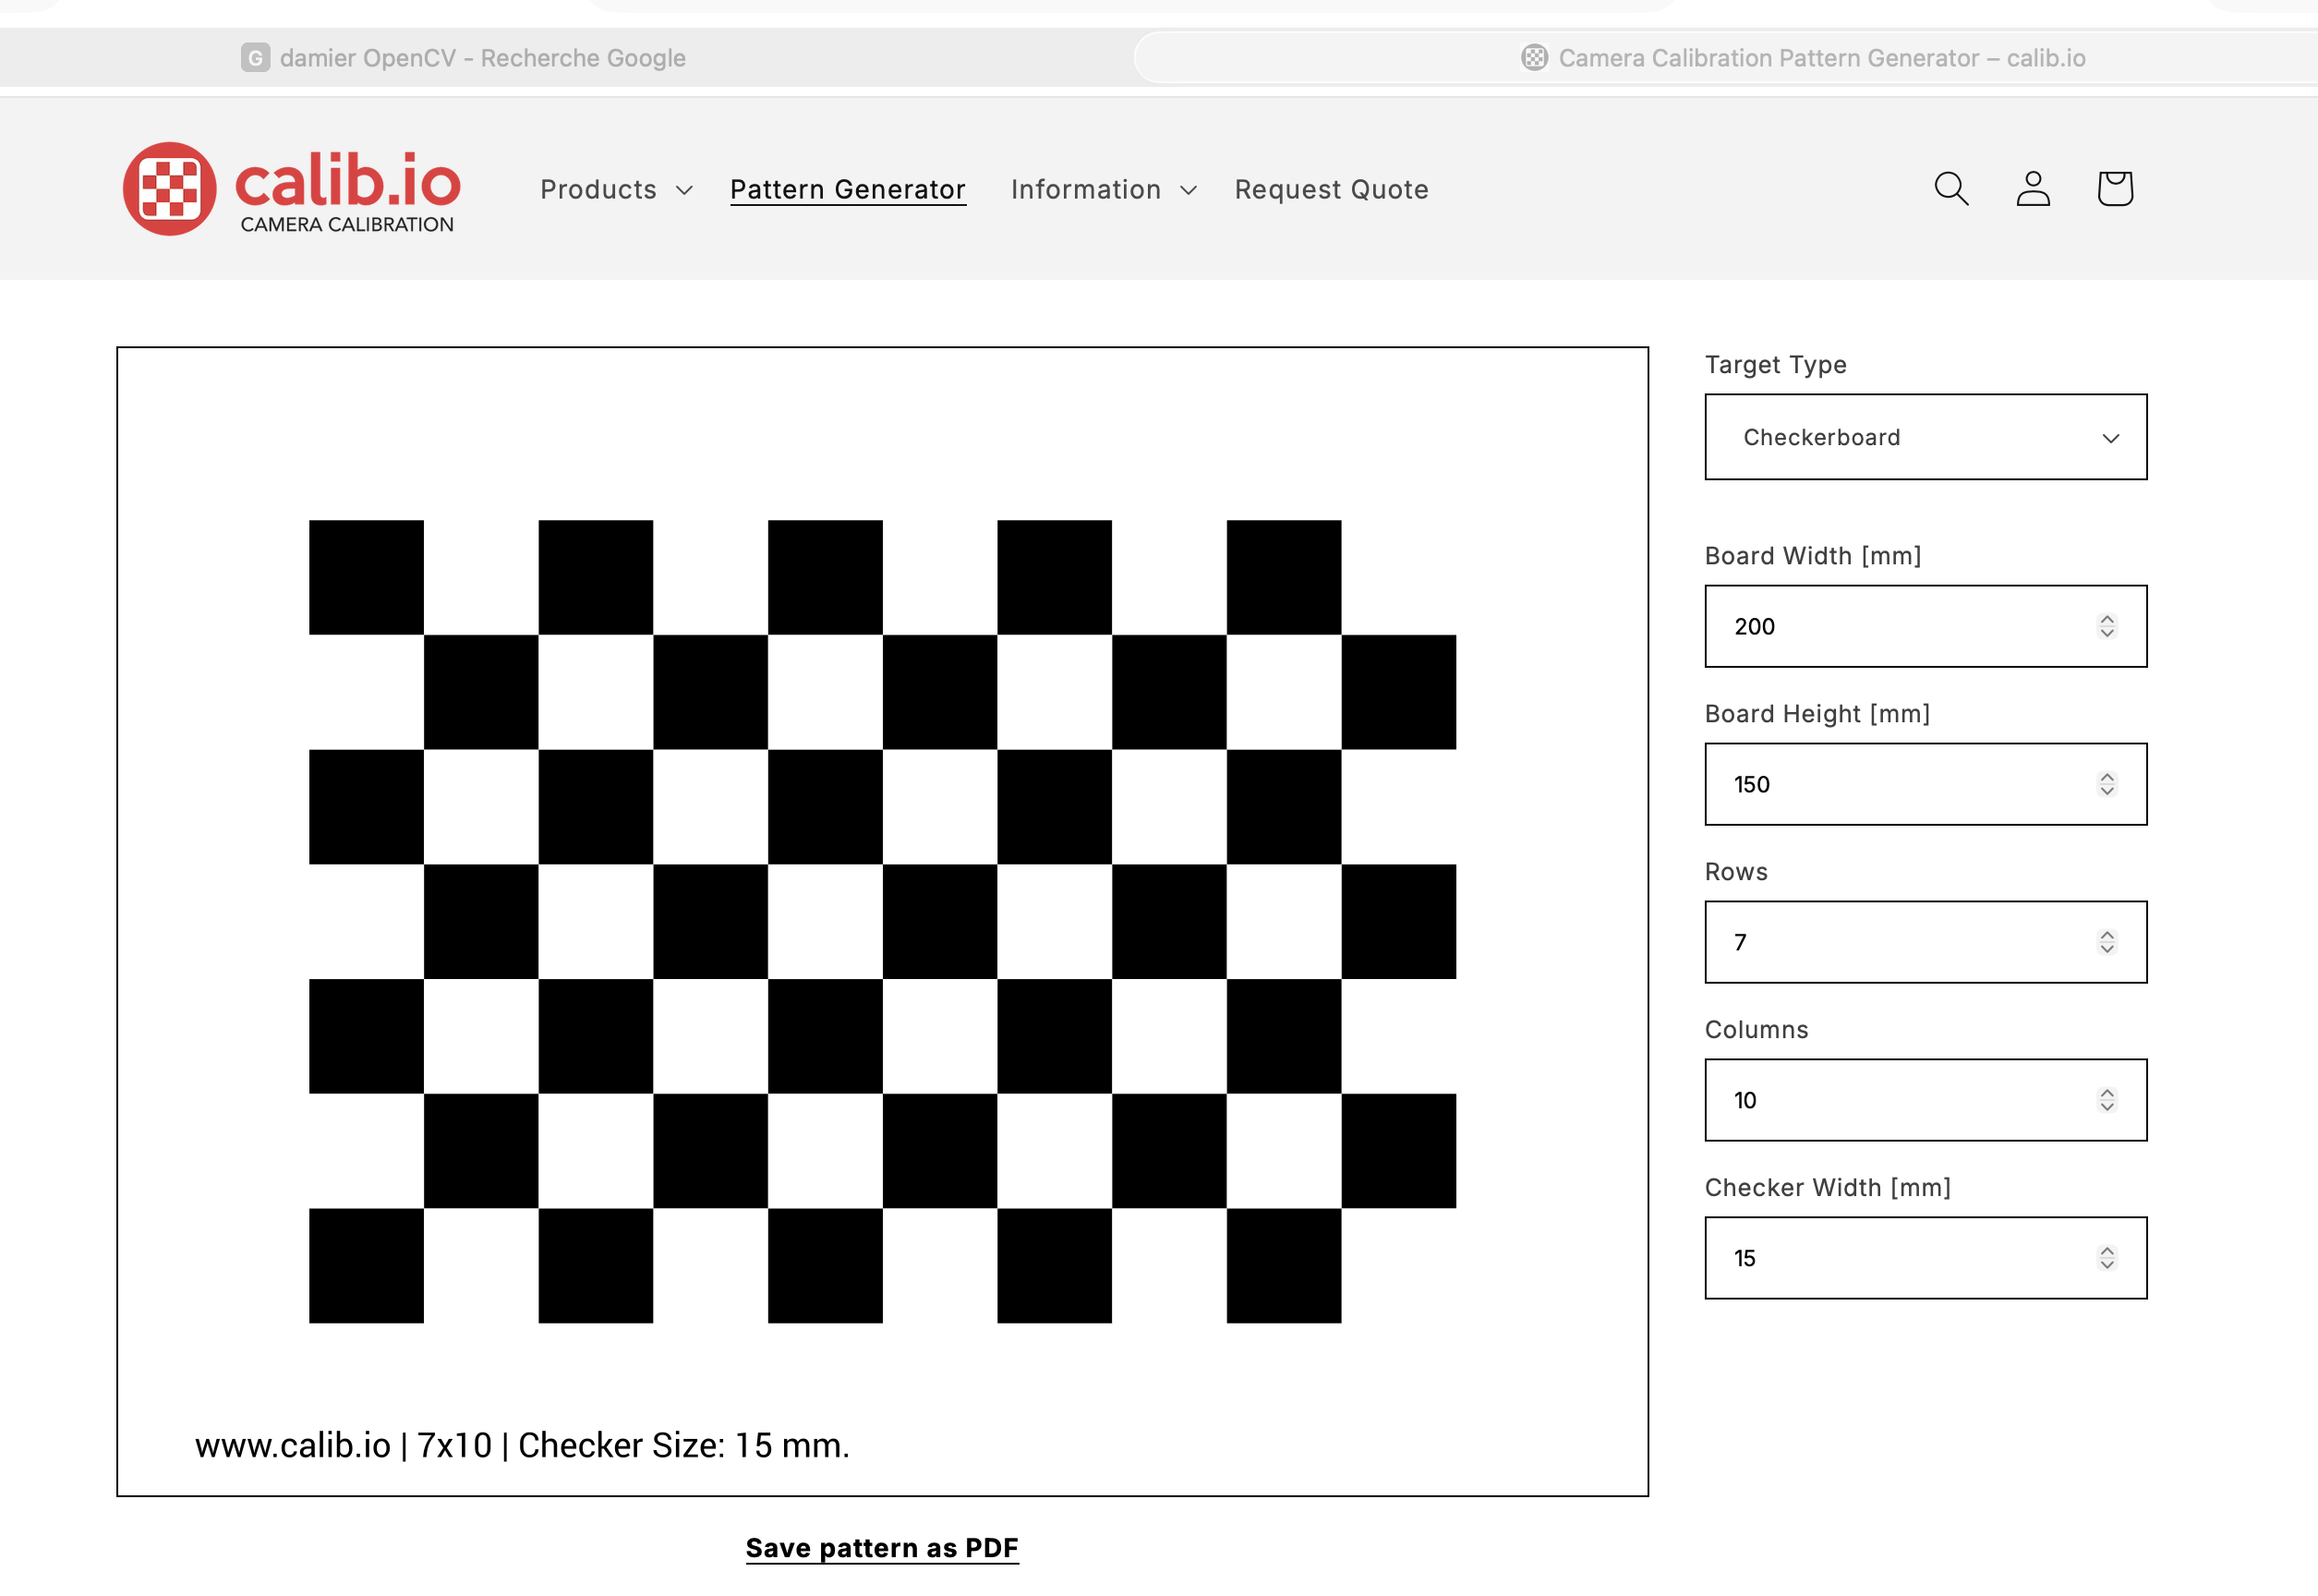
\includegraphics[width=0.75\textwidth]{preparation_motif_du_calibration.png}
    \caption{Interface de génération du motif sur \texttt{calib.io} spécifiant la grille $7 \times 10$ et la taille théorique de $15\text{ mm}$.}
    \label{fig:calib_io}
\end{figure}

\subsection{Affichage sur Écran et Mesure Métrique Directe}
Le motif généré a été affiché en plein écran sur un moniteur afin d'exploiter la planéité physique de la dalle. En raison du facteur d'échelle lié à la densité de pixels de l'écran (DPI), la dimension physique du carré a été mesurée directement sur la dalle à l'aide d'une règle millimétrée :
\[
S_{\text{réel}} = 0{,}85\text{ cm} = \mathbf{0{,}0085\text{ m}} \quad (\text{soit } 8{,}5\text{ mm})
\]
Cette valeur métrique exacte constitue l'échelle fondamentale pour le passage du repère pixel au monde 3D.

\subsection{Acquisition des 19 Clichés}
Un protocole rigoureux d'acquisition a été exécuté :
\begin{enumerate}
    \item \textbf{Nombre de vues :} 19 photographies acquises sans modifier la résolution ni la focale (autofocus verrouillé).
    \item \textbf{Variabilité spatiale :} Balayage complet des angles de tangage (\textit{pitch}), de roulis (\textit{roll}) et de lacet (\textit{yaw}), ainsi que variations de distance (près/loin) et décentrements vers les bords de l'image pour bien caractériser la distorsion radiale.
    \item \textbf{Qualité optique :} Baisse de la luminosité écran pour éliminer les reflets spéculaires et les artefacts de Moiré.
\end{enumerate}

\section{Modélisation Géométrique \& Formulation Mathématique}

\subsection{Équation de Projection Perspective (Modèle Pinhole)}
La projection d'un point 3D exprimé en coordonnées homogènes $P^{(W)} = [X, Y, Z, 1]^T$ vers un pixel image $p^{(I)} = [u, v, 1]^T$ est modélisée par :
\[
s \cdot \begin{bmatrix} u \\ v \\ 1 \end{bmatrix} = M_{\text{int}} \cdot M_{\text{ext}} \cdot \begin{bmatrix} X \\ Y \\ Z \\ 1 \end{bmatrix}
\]
où $s$ est un facteur d'échelle scalaire, $M_{\text{ext}} = [R \mid T]$ représente la matrice des paramètres extrinsèques ($3 \times 4$), et $M_{\text{int}}$ la matrice intrinsèque ($3 \times 3$) :
\[
M_{\text{int}} = \begin{bmatrix} f_x & 0 & O_x \\ 0 & f_y & O_y \\ 0 & 0 & 1 \end{bmatrix}
\]
avec $f_x, f_y$ les focales exprimées en pixels et $(O_x, O_y)$ le centre optique principal.

\subsection{Modélisation de la Distorsion Optique}
Les imperfections physiques de la lentille sont corrigées via les polynômes de distorsion radiale ($k_1, k_2, k_3$) et tangentielle ($p_1, p_2$) :
\[
x_{\text{corr}} = x (1 + k_1 r^2 + k_2 r^4 + k_3 r^6) + 2 p_1 x y + p_2 (r^2 + 2 x^2)
\]
\[
y_{\text{corr}} = y (1 + k_1 r^2 + k_2 r^4 + k_3 r^6) + p_1 (r^2 + 2 y^2) + 2 p_2 x y
\]

\section{Résultats de Calibration \& Analyse Métrique}

\subsection{Matrice Intrinsèque et Distorsion Estimées}
L'exécution du pipeline Python/OpenCV sur les **19 images validées ($100\%$ de taux de détection)** fournit les résultats suivants :

\begin{tcolorbox}[title=Résultats d'Étalonnage Globaux]
\textbf{Erreur de rétroprojection RMS :} $2{,}4210\text{ pixels}$.\\[0.2cm]
\textbf{Matrice Intrinsèque ($K$) :}
\[
K = \begin{bmatrix} 1526{,}38 & 0 & 1070{,}38 \\ 0 & 1547{,}41 & 794{,}51 \\ 0 & 0 & 1 \end{bmatrix}
\]
\textbf{Coefficients de distorsion :}
\[
[k_1, k_2, p_1, p_2, k_3] = [0{,}1088, -0{,}5957, 0{,}0156, 0{,}0216, 1{,}0892]
\]
\end{tcolorbox}

\subsection{Extraction de la Focale Physique en Mètres via \texttt{calibrationMatrixValues()}}
En injectant les dimensions physiques estimées du capteur ($4{,}8\text{ mm} \times 3{,}6\text{ mm}$), la fonction \texttt{cv2.calibrationMatrixValues()} permet d'isoler la grandeur métrique réelle demandée :

\begin{table}[ht!]
\centering
\caption{Synthèse des métriques physiques extraites.}
\vspace{0.2cm}
\begin{tabular}{ll}
\toprule
\textbf{Paramètre Physique} & \textbf{Valeur Extraite / Calculée} \\
\midrule
\textbf{Longueur Focale Physique ($f$)} & \textbf{$4{,}79\text{ mm}$ ($0{,}004789\text{ mètre}$)} \\
Champ de Vision Horizontal (FOV X) & $51{,}80^\circ$ \\
Champ de Vision Vertical (FOV Y) & $66{,}01^\circ$ \\
Point Principal $(O_x, O_y)$ & $(1070{,}38, 794{,}51)\text{ pixels}$ \\
Rapport d'Aspect (Aspect Ratio) & $1{,}0138$ (pixels quasiment carrés) \\
\bottomrule
\end{tabular}
\end{table}

\noindent \textbf{Analyse :} La focale calculée d'environ $4{,}79\text{ mm}$ correspond exactement aux spécifications matérielles des objectifs grands-angles équipant les smartphones modernes.

\section{Estimation de Pose 3D (PnP) \& Application AR}

Une fois la matrice $K$ et la distorsion connues, l'algorithme \texttt{cv2.solvePnP()} résout le problème de la pose pour déterminer la rotation $R$ et la translation $T$ de la caméra par rapport au damier. Un repère orthonormé $3\text{D}$ (Axes $X$ rouge, $Y$ vert, $Z$ bleu de longueur $3 \times S_{\text{réel}}$) est projeté à l'origine du damier via \texttt{cv2.projectPoints()}.

\begin{figure}[ht!]
    \centering
    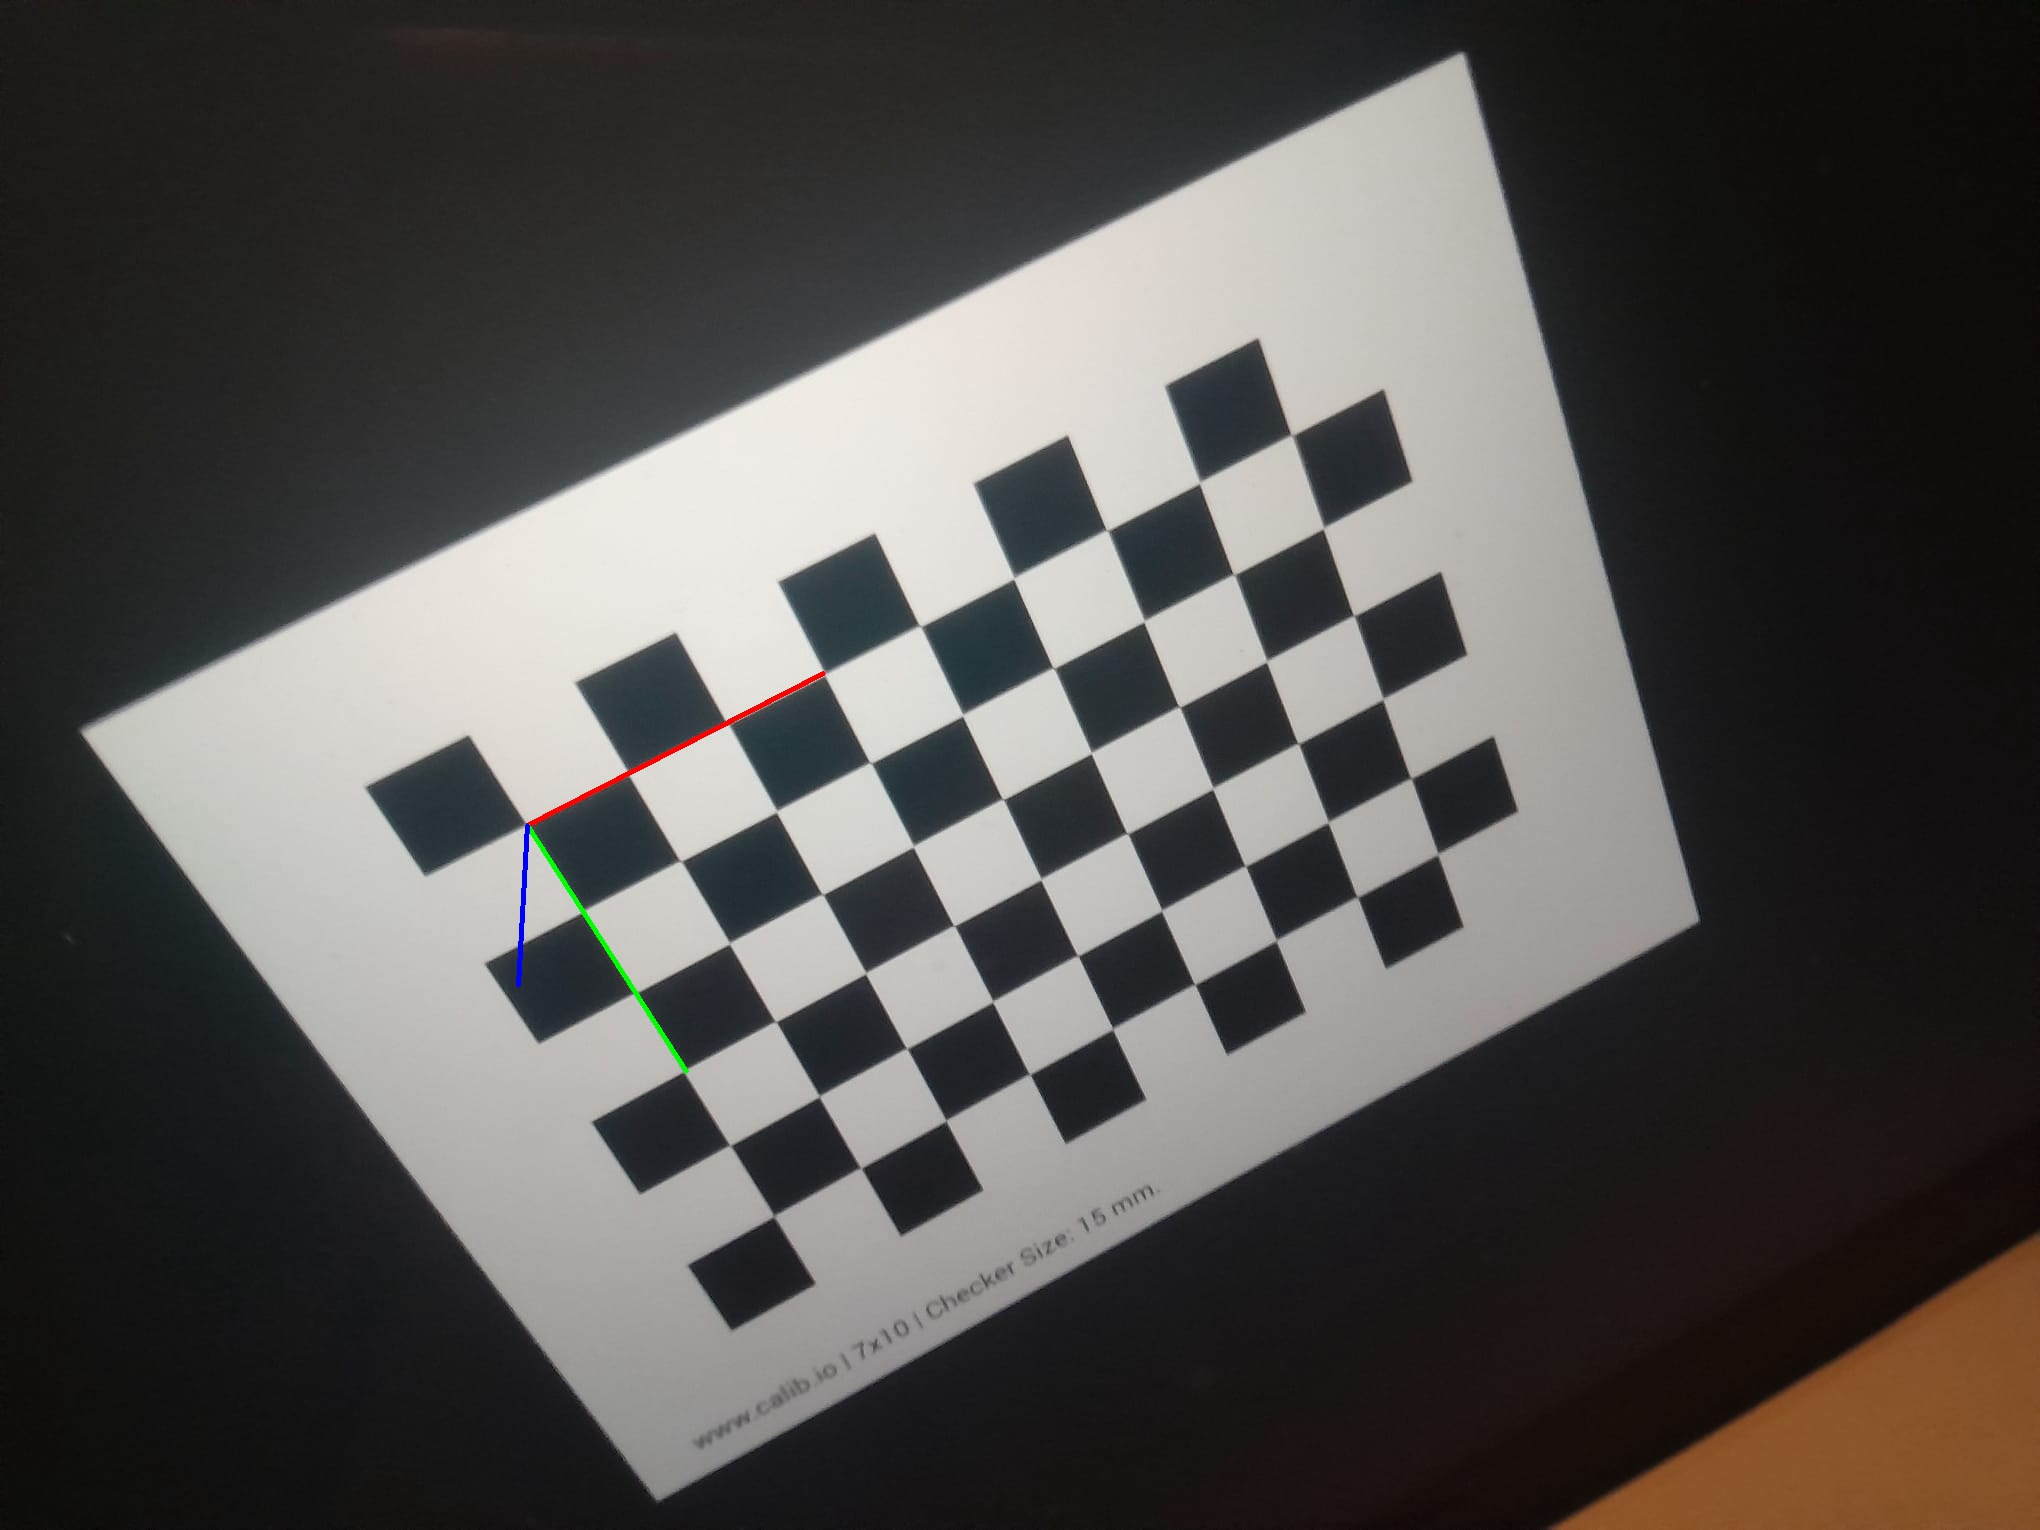
\includegraphics[width=0.65\textwidth]{../data/output/pose_3d_resultat.jpg}
    \caption{Projection tridimensionnelle des axes de coordonnées en réalité augmentée au coin du damier.}
    \label{fig:pose3d}
\end{figure}

\section{Discussion \& Analyse des Sources d'Erreur}

\begin{itemize}
    \item \textbf{Explication de l'erreur RMS ($2{,}42\text{ px}$) :} L'erreur de rétroprojection est légèrement supérieure à celle obtenue sur papier imprimé. Cela s'explique par la nature du support d'affichage (matrice de sous-pixels de l'écran créant un léger flou de réfraction et des phénomènes de Moiré lors de la détection sub-pixellique).
    \item \textbf{Qualité de la planéité :} L'utilisation de l'écran offre en contrepartie une planéité absolue ($Z=0$), éliminant tout biais lié aux pliures d'une feuille de papier.
\end{itemize}

\end{document}